\documentclass{cmspaper}
\usepackage{booktabs}
\usepackage{graphicx}
\usepackage{rotating}


\begin{document}

\def \mrad      {{\rm \, mrad}}
\newcommand {\cm}         {\rm   cm}
\newcommand {\mm}         {\rm   mm}
\newcommand {\m}          {\rm   m}

\renewcommand{\labelenumi}{\alph{enumi})}
\newcommand{\fixme}{{\bf FIXME~}}


%==============================================================================
% title page for few authors

\begin{titlepage}

% select one of the following and type in the proper number:
%   \cmsnote{2005/000}
  \internalnote{2008/000}
%  \conferencereport{2005/000}
   \date{1 April 2008}

  \title{Tracker Inner Barrel and Inner Disks\\
  Geometry and Material Budget}

  \begin{Authlist}
    Ernesto Migliore
     \Instfoot{to}{INFN Torino}
    Giacomo Sguazzoni
     \Instfoot{fi}{INFN Firenze}
  \end{Authlist}

 
  \begin{abstract}
This internal note contains the release notes of the Geometry and
Material Budget of TIB and TID in CMSSW 2.0.x cycle. 
%This major update concerns the passive material of TIB and TID services that are thoroughly described. 
  \end{abstract} 

\end{titlepage}

\setcounter{page}{2}%JPP

This document describes the implementation into the CMSSW software of
the Geometry and of the Material Budget of the inner parts of the
Silicon Strip Tracker, namely the Tracker Inner Barrel (TIB), the
Tracker Inner Discs (TID) and the TIB/TID services, the
latter being accounted for up the end of the Tracker Support Tube (TST).
\fixme: add $z$ range, describe the remaining path to PP1.
In the following, TIB, TID and TIB/TID services will be called for
simplicity Inner Tracker.

The current description is the outcome of the review of the Material
Budget of the CMS Tracker carried on during 2007. This review work
affected the description of the detector both in terms of introducing
new elements and of modifying the geometry and the material of those
already existing.

Therefore the present version of the geometry is a substantial update of the description
of the Tracker which, at the beginning of the review, was in several
aspects that corresponding to the hardware configuration described in the Tracker TDRs~\cite{tdr}.

The description of the TIB, TID and their services in the CMS software
is based on the GEANT4 toolkit~\cite{geant4} and it is accomplished using the
Detector Description Language~\cite{ddl}. The implementation of the
tree of the Logical Volumes was done following
the general guidelines described in~\cite{rrValid}. 

In implementing the description the following considerations were
taken into account:
\begin{itemize}
\item most of the components of the TIB and of the TID were built
  following the same specifications (same functional layout, same material
  used both in terms of chemical composition and of mechanical
  arrangement, same population of sub-components) differing in
  the realization to account for the different topology of the
  barrel cylindrical shells or of the endcap discs;
\item TIB and TID share in practice all the services (power and control
  cables, ribbons of signal and control optical fibers, cooling pipes).
\end{itemize}
The first consideration is reflected in the code organization by the
fact that the same model for describing components
which are in common to TIB and TID was adopted  thus using the same materials when
not even the same Logical Volumes~\footnote{In GEANT4 Logical Volumes
  are the objects which manage the information associated with
  detector elements represented by a given Solid and Material,
  independently from its physical position in the detector, 
  while Physical Volumes represent the spatial positioning of the
  volumes describing the detector elements.}. 
The list of admixtures describing composite materials used both in the
TIB and the TID is given in Table~\ref{tab:tibtid_common}.\\ 
Because of the second one, starting from the releases of the 1.6.x cycle
only two mother Logical Volumes were defined to
group all the services not mounted directly on the surfaces where the
active elements (sensors) are for the forward and the backward parts 
called {\tt TIBTIDServicesF} and {\tt TIBTIDServicesB} respectively.

\begin{table}[h!]
  \caption{Admixtures for composite materials used in common in TIB
  and TID Logical Volumes. \fixme Togliere ``Norm.''}
  \label{tab:tibtid_common}
  \begin{center}
    \begin{tabular}{llccc}
Name         & Description & Norm. density [g/cm$^3$] & Norm. X$_0$ [cm] & Norm. $\lambda_0$ [cm] \\
\hline
TIBTID\_CCUM & CCUM    &                0.81143 &        22.89567 &       112.26978 \\
TIBTID\_DOH  & DOH     &                0.79092 &        23.10703 &       119.21202 \\
TIBTID\_PA   & PA per cm$^2$  &         2.74978 &         9.90981 &        34.36277 \\
TIBTID\_AOH  & AOH            &         0.60091 &        30.49142 &       155.66922 \\
TIBTID\_AmphCable & Amphenol cable 26cond per cm  &   2.05153  & 9.05980 &        46.00076 \\
TIBTID\_HybridBoard & TIB TID Hybrid Board  &         3.70257 &         5.82843 &        27.52748 \\
TIBTID\_HybridTails   & TIB TID Hybrid Tails &         1.61323 &        13.92045 &        55.22686 \\
TIBTID\_Hybrid        & TIB TID Hybrid  &         2.16228 &         9.78741 &        47.54797 \\
\hline
    \end{tabular}
  \end{center}
\end{table}

%%%%%%%%%%%%%%%%%%%%%%%%%%%%%%%%%%%%%%%%%%%%%%%%%%%%
\section{Review of the TIB, TID active volumes}
%%%%%%%%%%%%%%%%%%%%%%%%%%%%%%%%%%%%%%%%%%%%%%%%%%%%
\fixme questa sezione potrebbe anche essere rimossa. Provare a mettere
figure ottenute con il tool di confronto delle geometrie

%%%%%%%%%%%%%%%%%%%%%%%%%%%%%%%%%%%%%%%%%%%%%%%%%%%%
\section{Review of the TIB, TID passive volumes}
%%%%%%%%%%%%%%%%%%%%%%%%%%%%%%%%%%%%%%%%%%%%%%%%%%%%
A correct description of the material budget of the detector should lead
to perturbations of the state of a simulated particle which are on average equal
to those found in the data.  
In absence of data from collisions, the leading criterium for tuning of
the detector effects is to have the mass of the detector described in
the simulation as close as possible to the real one.
In this respect both a ``bottom-up'' and a ``top-down'' review of the mass
of the components were performed.
\subsection{The ``bottom-up'' approach}
The granularity of the volumes as implemented in the releases of the
2.0.x cycle is shown in Figure~\ref{fig:tibtid_pv_size} where the multiplicity of the
different Physical Volumes as a function of 1/$X_0$, which is
proportional to the photon conversion probability, and the size of
the volume itself is shown. Different categories of volumes can be
identified: elements with a multiplicity scaling as the number of the
{\it Modules}, O(10000),  elements with multiplicity scaling as the number
of the {\it Strings}, O(1000), elements with multiplicity scaling as the
number of the {\it Control Rings}, O(100), and elements with multiplicity
scaling as the number of the {\it Mechanical Structures}, O(10). 
\begin{figure}[hbtp]
  \begin{center}
  \resizebox{0.7\linewidth}{!}{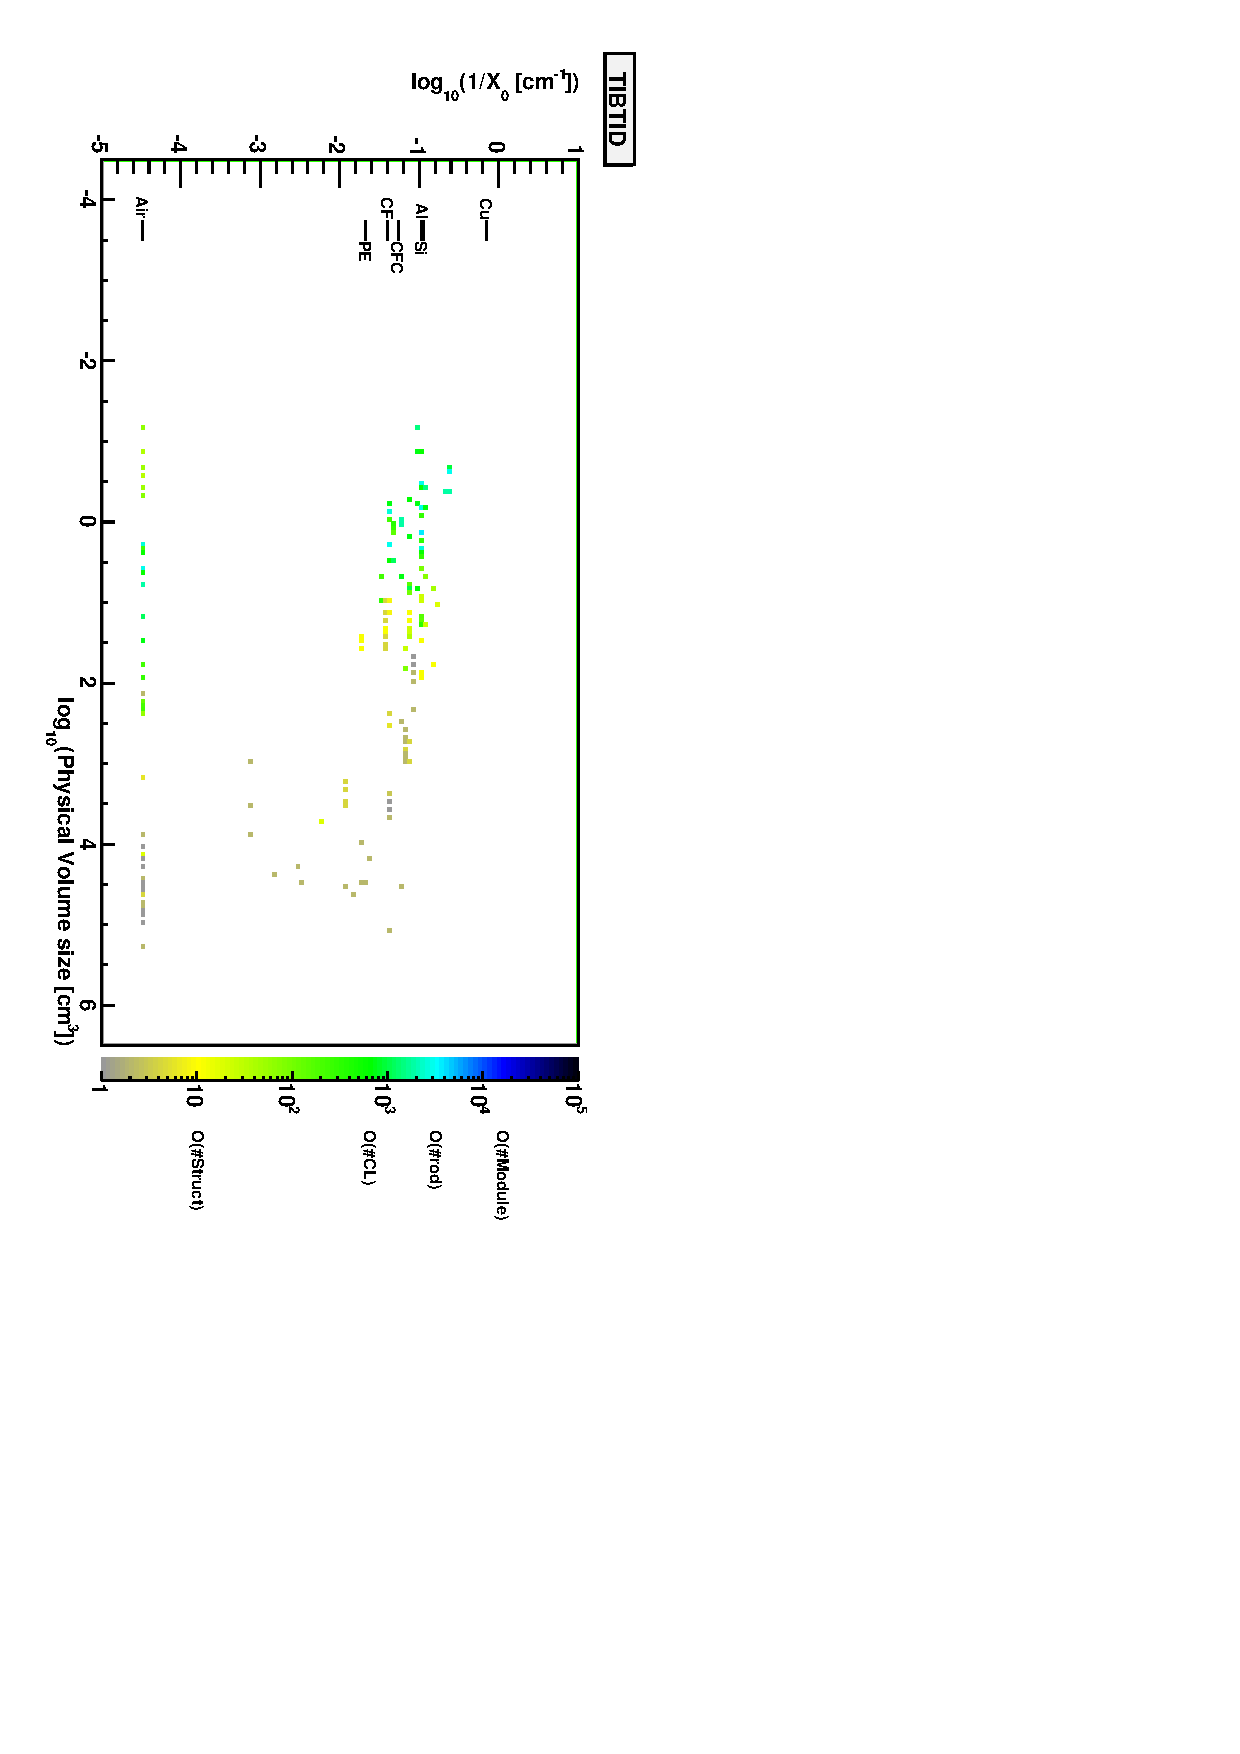
\includegraphics[angle=90]{TIBTID_PV_Size_Log.pdf}} 
    \caption{Number of instances of Inner Tracker Physical Volumes in
      the (volume,1/$X_0$) plane. 1/$X_0$ values for common materials are indicated on the
    left. \fixme old version}
    \label{fig:tibtid_pv_size}
  \end{center}
\end{figure}
In the following the description of the components in
order of descending multiplicity is presented. A separate section is devoted to the
description of the services.

\subsubsection{Elements with the multiplicity of the Modules}
\paragraph{Modules}
\begin{figure}[hbtp]
  \begin{center}
  \resizebox{0.7\linewidth}{!}{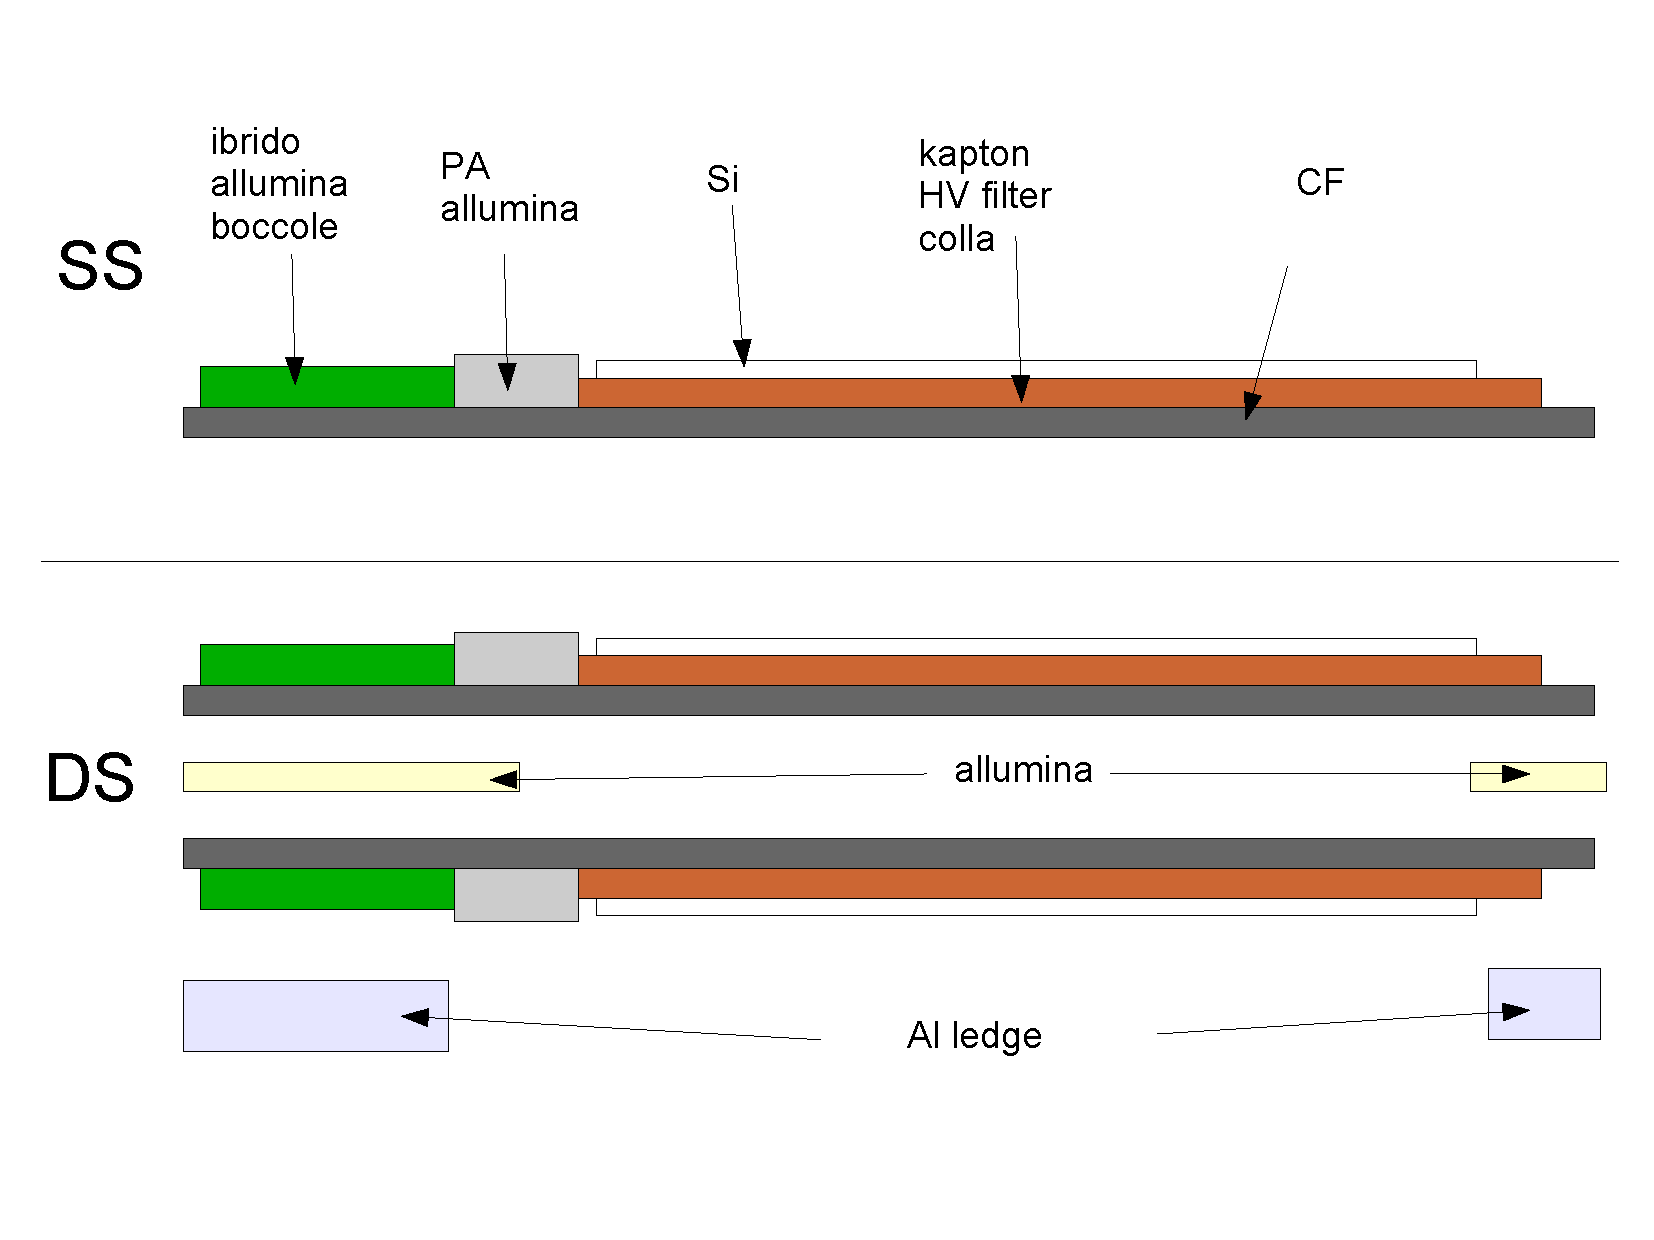
\includegraphics{sketch_modulo.pdf}} 
    \caption{}
    \label{fig:module}
  \end{center}
\end{figure}
TIB and TID modules were designed and built with the same layout
differing only in the geometry of some of the components, rectangular-shaped
for the barrel and wedge-shaped for the discs.
Therefore in the simulation the same tree of volumes was used for the
description of TIB and TID modules. 
%The description of the modules is a balance between accuracy and the
%simplicity of the code
The volumes used to describe TIB/TID modules are shown
Figure~\ref{fig:module}: Double-Sided modules are 
formed by a double replica of the volumes of the Single-Sided modules,
with the proper geometrical differences between the $r\phi$ and stereo sides,
with the addition of extra volumes for the ceramic spacers in between. 
The volumes corresponding to the aluminum ledges,
which are the pieces where modules are mounted on the cooling pipes, were also
included in the  {\tt Module} mother volume~\footnote{Actually 3 types
  of modules were defined for the TIB ({\tt TIBModule0A}, B, {\tt
    TIBModule0B} and {\tt TIBModule2}) and 5 for the TID ({\tt
    TIDModule0L}, {\tt TIDModule0R}, {\tt TIDModule1L}, {\tt
    TIDModule1R} and {\tt TIDModule2}).}. 
The reason of this choice was to guarantee an accurate description of
these localized amounts of material close to the active areas. 
Most of the volumes (sensor, frame, pitch-adapter, ceramic spacer,
aluminum ledges) correspond to elements containing in reality just one
or two materials. Therefore they were implemented in the simulation
using the geometry and the materials from the engineering drawings.
The volumes corresponding to the carbon fiber frame were actually
segmented along the local $v$ direction to account the rather
complicated shape of the real frames. 

Concerning the front-end hybrids, they were included, both for the TIB
and for the TID, in the volume of the modules for the part glued on
the carbon fiber frame.  
This volume was filled by the same admixture both for TIB and for TID
hybrids determined from the specifications of~\cite{hybrid}.
The amount of copper in the layer containing the traces was assumed to
be 7\% of that in the power planes to match the mass measured on (one) spare hybrids.
The number of APV chips used in the definition of the admixture was
5.2 per module which is the average values for 4/6 APV modules in the
Inner Tracker (Table~\ref{tab:apv}). The same value was used to compute the
contribution of SMD components (capacitors and resistors) scaling with the
number of APVs. 
\begin{table}[h!]
  \caption{Number of 4/6 APV modules in TIB and TID.}
  \label{tab:apv}
  \begin{center}
    \begin{tabular}{lcc}
      & 4 APVs & 6 APVs \\
      \hline
      TIB& 1188& 1536 \\
      TID&  240&  576 \\
      \hline
    \end{tabular}
  \end{center}
\end{table}
A separate volume, not included in the {\tt Module} volume, was
defined containing the ``tails'' and the connectors for the low
voltage/control lines and the analog readout.  

In figure~\ref{fig:TIDModule} the real TID modules and their actual description in
the simulation are compared. The simplifications used in the simulation
are visible. The guideline in defining the simulated geometry
was to recover the value of the carbon fiber frame area as determined from the
engineering drawings. 

The detailed lists of the volumes forming the TIB and the TID modules
are given in Tables~\ref{tab:tib_module} and~\ref{tab:tid_module}.  
The agreement between the measured and simulated mass of the module is
order of 1 g (cf. Table~\ref{tab:tibtid_module_mass}).   
\begin{table}[h!]
  \caption{Measured and simulated mass of TID modules. The mass of the
  measured hybrid ``tails'' was subtracted to the measured mass and
  that of the aluminum ledges was subtracted from the simulated.
  Multiplicity is in TIDF and TIDB}
  \label{tab:tibtid_module_mass}
  \begin{center}
    \begin{tabular}{lccc}
      & Measured Mass [g] & Simulated Mass [g] & Mult.\\
      \hline
      {\tt TIDModule0*} & 44.9 & 45.65 & 144 \\
      {\tt TIDModule1*} & 45.8 & 47.95 & 144 \\
      {\tt TIDModule2}  & 17.5 & 17.22 & 240 \\
      \hline
    \end{tabular}
  \end{center}
\end{table}

\paragraph{Analog Opto-Hybrids (AOHs)}

\subsubsection{Elements with the multiplicity of the Strings}
\paragraph{Mother-Cables} 
TIB/TID mother-cables are the electronic boards providing low voltage
and high voltage lines to the modules and connecting the modules to the CCU.\\

\fixme TIB\\

In the real TID there are 4 mother-cables on each side of each Ring for a
total of 5 different ``sickle-like'' geometries: 2 different
geometries (A, B) for the Ring1 and
Ring3 and 1 geometry for the Ring2. The description in the simulation
was simplified implementing the mother-cables on each side of a Ring
as a $\phi=2\pi$ ring, with the radial dimensions taken from the
engineering drawings, plus 4 radial rectangular arms. 
Concerning their composition, the real TID mother-cables are kapton
multilayer-boards with 3 copper layers for the ground and power planes and 2 for
the traces. In the CMSSW description the same amount of copper per
unit surface was assumed for all the 3 rings and for the rectangular arms.
The correct number of IC and SMD components was put in each of the 3 admixtures
representing the mother-cables of each Ring.

A comparison of real and simulated mass of the 4 mother-cables present
on one side of the 3 different Rings is given in Table~\ref{tab:tid_mc}.
\begin{table}[h!]
  \caption{Measured and simulated mass of the TID mother-cables on one
  side of a Ring.  Multiplicity is in TIDF and TIDB. The CCU socket is
  included in the masses but not the CCU chip.}
  \label{tab:tid_mc}
  \begin{center}
    \begin{tabular}{lccc}
      & Measured Mass [g] & Simulated Mass [g] & Mult. \\
      \hline
      Ring1 & 196.6 & 200.32 & 12 \\
      Ring2 & 203.6 & 213.99 & 12 \\
      Ring3 & 230.4 & 250.47 & 12 \\
      \hline
    \end{tabular}
  \end{center}
\end{table}


\subsubsection{Elements with the multiplicity of the Control Rings}
\paragraph{Digital Opto-Hybrids Modules (DOHMs)}
The TIB/TID DOHMs are the master cards of each control-ring. They are
multilayer PCB boards housing 2 DOHs and the CCU which implements the
redundancy logic of the control-ring.
The number of ancillary elements depends on the number of
mother-cables connected to the DOHM, 7 for the TIB  and 4 for
the TID. \fixme auxiliary for TIB.

In the TID there are two different DOHM geometries: one in common to Ring1 and
Ring2 and a larger one for Ring3.
There are 2 DOHM boards for each Ring of the TID.\\
Since TIB and TID DOHMs were produced by different manufacturers
different admixtures were used in describing TIB and TID DOHMs.

TID DOHMs were implemented in volumes reproducing those of the actual
DOHM boards as determined on a 3D-measurement machine.
The board was modeled as made of FR4 with 6 copper layers, each 35
$\mu$m thick. The ground and the power layers were assumed to be entirely filled by
copper while the 4 signal layers were assumed to be filled by copper
for the same fraction of surface as they are filled in the TIB DOHMs. 
The correct number of connectors, IC and SMD components was put in
each of the 2 admixtures representing the DOHMs of Ring1/Ring2 and Ring3 respectively.

A comparison of real and simulated mass of the two different DOHM
boards is given in~\ref{tab:tid_dohm}.
\begin{table}[h!]
  \caption{Measured and simulated mass of the TID DOHMs.  Multiplicity is in TIDF and TIDB.}
  \label{tab:tid_dohm}
  \begin{center}
    \begin{tabular}{lccc}
      & Measured Mass [g] & Simulated Mass [g] & Mult.\\
      \hline
      Ring1/Ring2 & 52.5 & & 12 \\
      Ring3       & 71.6 & & 12 \\
      \hline
    \end{tabular}
  \end{center}
\end{table}

\paragraph{Cooling Pipes}
\paragraph{Cooling Manifolds}
\subsubsection{Elements with the multiplicity of the Mechanical Support Structures}

\subsection{TIB/TID Services}
%%%%%%%%%%%%%%%%%%%%%
\input ./services.tex
%%%%%%%%%%%%%%%%%%%%%%
\pagebreak
%%%%%%%%%%%%%%%%%%%%%%%%%%%%%%%%%%%%%%%%%%%%%%%%%%%%
\section{The ``top-down'' approach}
%%%%%%%%%%%%%%%%%%%%%%%%%%%%%%%%%%%%%%%%%%%%%%%%%%%%
The masses of the forward and of the backward halves of the Inner
Tracker were measured independently at the Tracker Integration
Facility (TIF) during the insertion in the Tracker Outer Barrel (TOB)
in the Fall 2006. 
The instrument used was an analog PIAB dynamometer~\cite{piab}  of
2000 kg capacity, a display with 20 kg graduation and an accuracy of
$\pm$0.6\% of the maximum capacity. 
Each weighted half consisted of: 
\begin{enumerate}
\item half TIB  
\item forward/backward TID enclosed in the Service Cylinder
\item services described in the previous section up to the Margherita
  panel (included)
\item paths of ribbons of fibers to be laid along the TST and hanging on the
Margherita 
\item a cradle housing the detector for the transportation. 
\end{enumerate}
The cooling pipes were emptied before moving the detector.
The obtained measurements were:
\begin{itemize}
\item forward: 840 - 520 (cradle) - 94 (tare) = 226 kg 
\item backward:
\end{itemize}
which give an overall (forward+backward) mass of 452 kg.
This value has to be compared with that obtained in the simulation
restricting to the volumes actually measured and after subtracting,
always in the simulation, the weight of the coolant. 
The latter was estimated from the Fluorine content  in the
{\tt volume.element} files produced by the standard CMSSW module {\tt
  SimG4Core/PrintGeomInfo/interface/MaterialBudgetInfo}.
The simulated mass was 333 kg (119 kg or 26\% discrepancy) in the
releases up to 1.6.x and it is  \fixme 416 kg (36 kg or 8\%
discrepancy) in the current one.
Detail of the evolution of the mass of the different volumes in the
different releases is shown in Table~\ref{tab:mass_version}

\begin{table}[h!]
  \caption{in kg }
  \label{tab:mass_version}
  \begin{center}
    \begin{tabular}{lrrrr}
%      \hline
        & \multicolumn{4}{c}{CMSSW release} \\
        &  1.4.x  &  1.6.x  &  1.7.x  &  2.0.x \\
       \hline
      {\tt TIB}            & 304 kg & 196 kg & 206 kg &  \\
      {\tt TIDF}+{\tt TIDB}            & 138 kg &  70 kg &  73 kg & \\
      {\tt TIBTIDServicesF}+{\tt TIBTIDServicesB} &  n.a.  & 408 kg & 409 kg & \\
%      \hline
      Sum            & 442 kg & 674 kg & 689 kg & \\
       \hline
      Weighted       & 333 kg & 403 kg & 415 kg & \\
      Missing        & 119 kg &  49 kg &  37 kg & \\
                     & -26.4\% & 10.8\% & 8.2\% &\\
       \hline
    \end{tabular}
  \end{center}
\end{table}

\subsection{Calibration of the analog dynamometer}
The calibration of the analog PIAB dynamometer was checked in Torino in November
2007 against a digital electronic dynamometer ABC~\cite{abc}.
The digital dynamometer has a capacity of 3200 kg, and a nominal
accuracy of 1 kg. The calibration procedure consisted in loading the
system shown in Figure~\ref{fig:TOsetup} with pairs of lead tiles of
about 2$\times$11 kg each, up to reach a payload of about 950
kg. Measurements were taken also during the descent curve (with a
coarser step) and when charging again the load up to about 250 kg.
For the test the digital dynamometer was zeroed with the analog
dynamometer suspended. The PIAB readouts were rounded at 5 kg.\\
Figure~\ref{fig:calib_line} shows the
values measured by the PIAB as a function of those measured by the ABC
dynamometer. The linearity (?) of the instrument was found to be within the percent
level but a global offset of up to about 10 kg on the individual PIAB
measurements was found. As the masses of the two halves were determined as a
difference of two measurements, the differences of all possible pairs of
analog measurements $\Delta_{\mathrm{PIAB}}$  were checked against the
corresponding difference of the digital instrument $\Delta_{\mathrm{ABC}}$.
The result is shown in Figure~\ref{fig:calib_delta}: the top plot
shows the distribution of the double difference
$\Delta_{\mathrm{PIAB}}-\Delta_{\mathrm{ABC}}$, the middle plot the
double difference as a function of $\Delta_{\mathrm{PIAB}}$ and the
bottom plot as a function of the mass of the payload measured by the
analog instrument. Despite the top distribution shows no bias and a
RMS of about 4 kg, the plot in the middle shows that for a single  
$\Delta_{\mathrm{PIAB}}$, in the region of interest for the Inner Tracker
measurement (550-650 kg), the ``double-difference'' is spread in a range
of $\pm$10 kg. Moreover, when examined as a function of the PIAB
measurement, $\Delta_{\mathrm{PIAB}}-\Delta_{\mathrm{ABC}}$ shows a
trend which reflects the granularity in the readouts of the PIAB (?).
Therefore $\pm$10 kg was assumed as error on the measurement of each
of the two Inner Tracker halves.

\begin{figure}[hbtp]
  \begin{center}
    \begin{tabular}{cc}
      \resizebox{0.4\linewidth}{!}{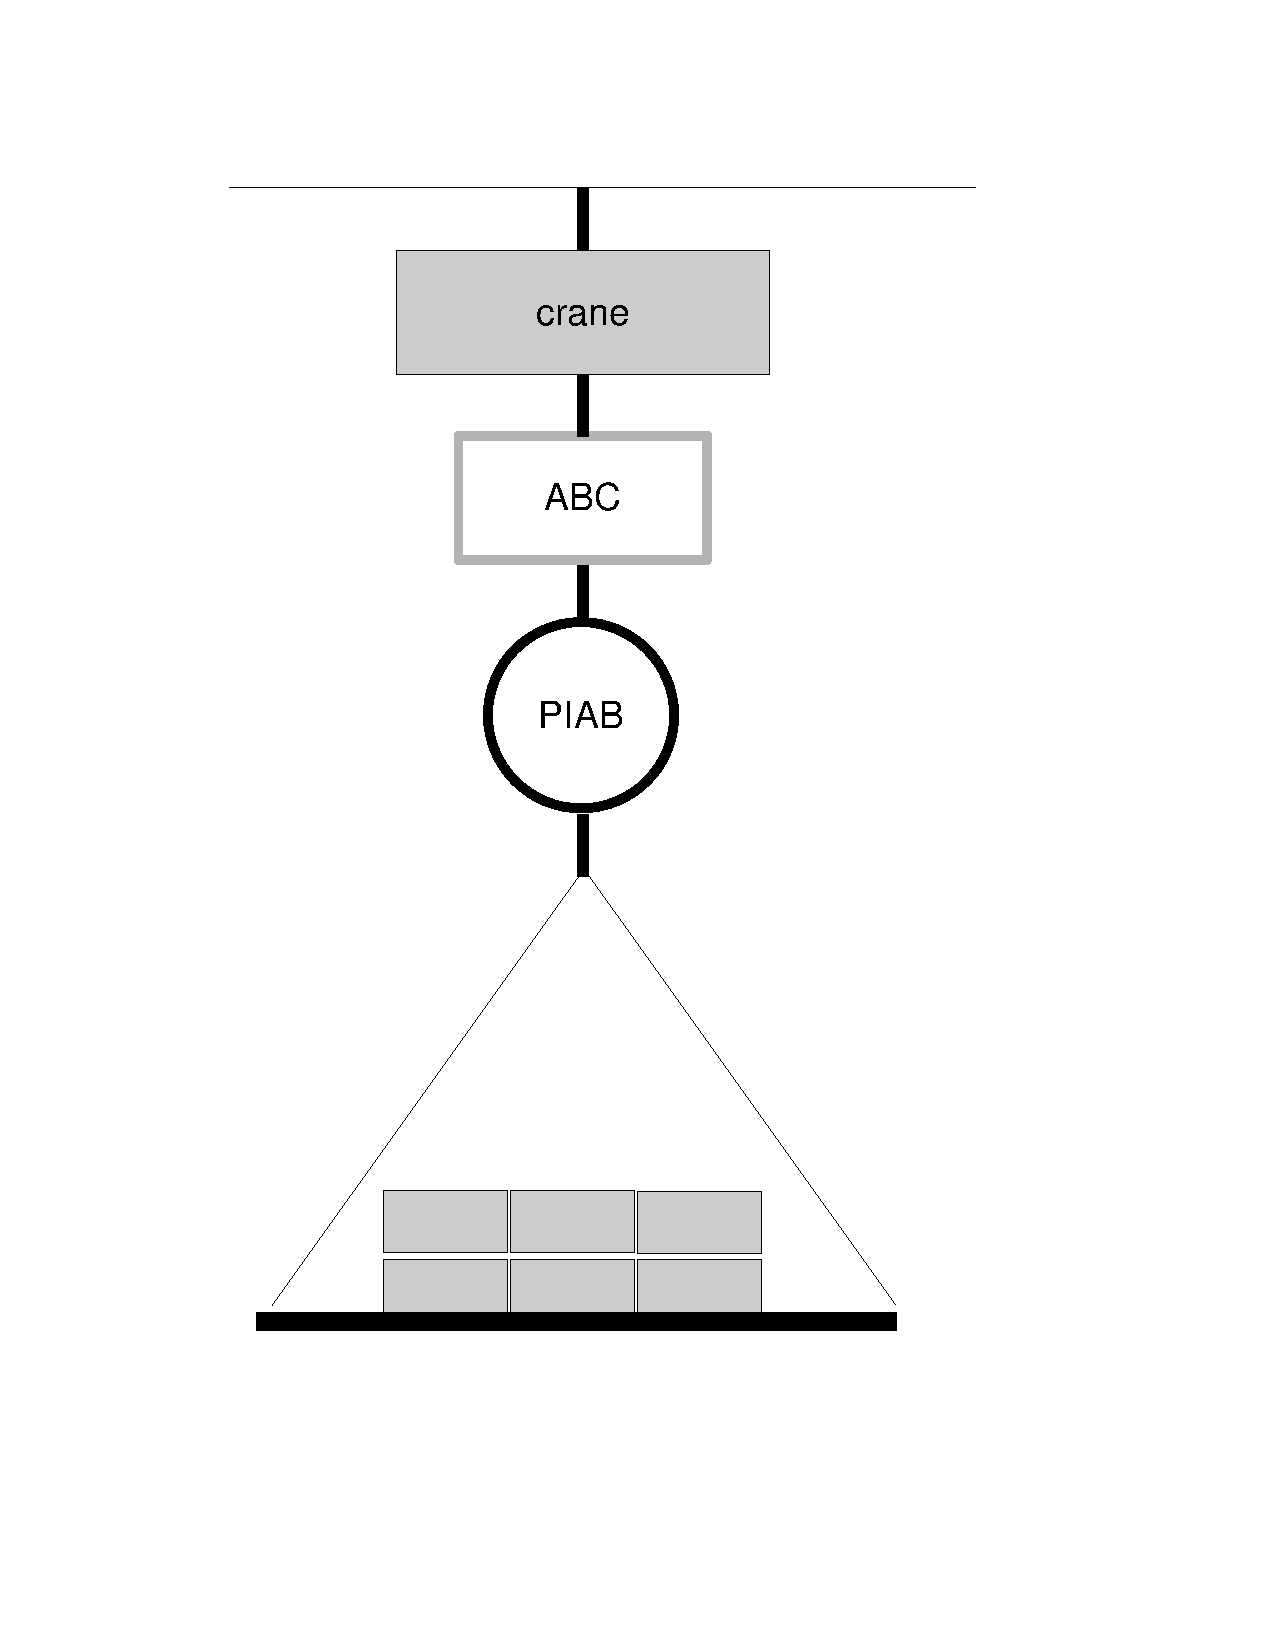
\includegraphics{TorinoSetup.pdf}}  &
      \resizebox{0.6\linewidth}{!}{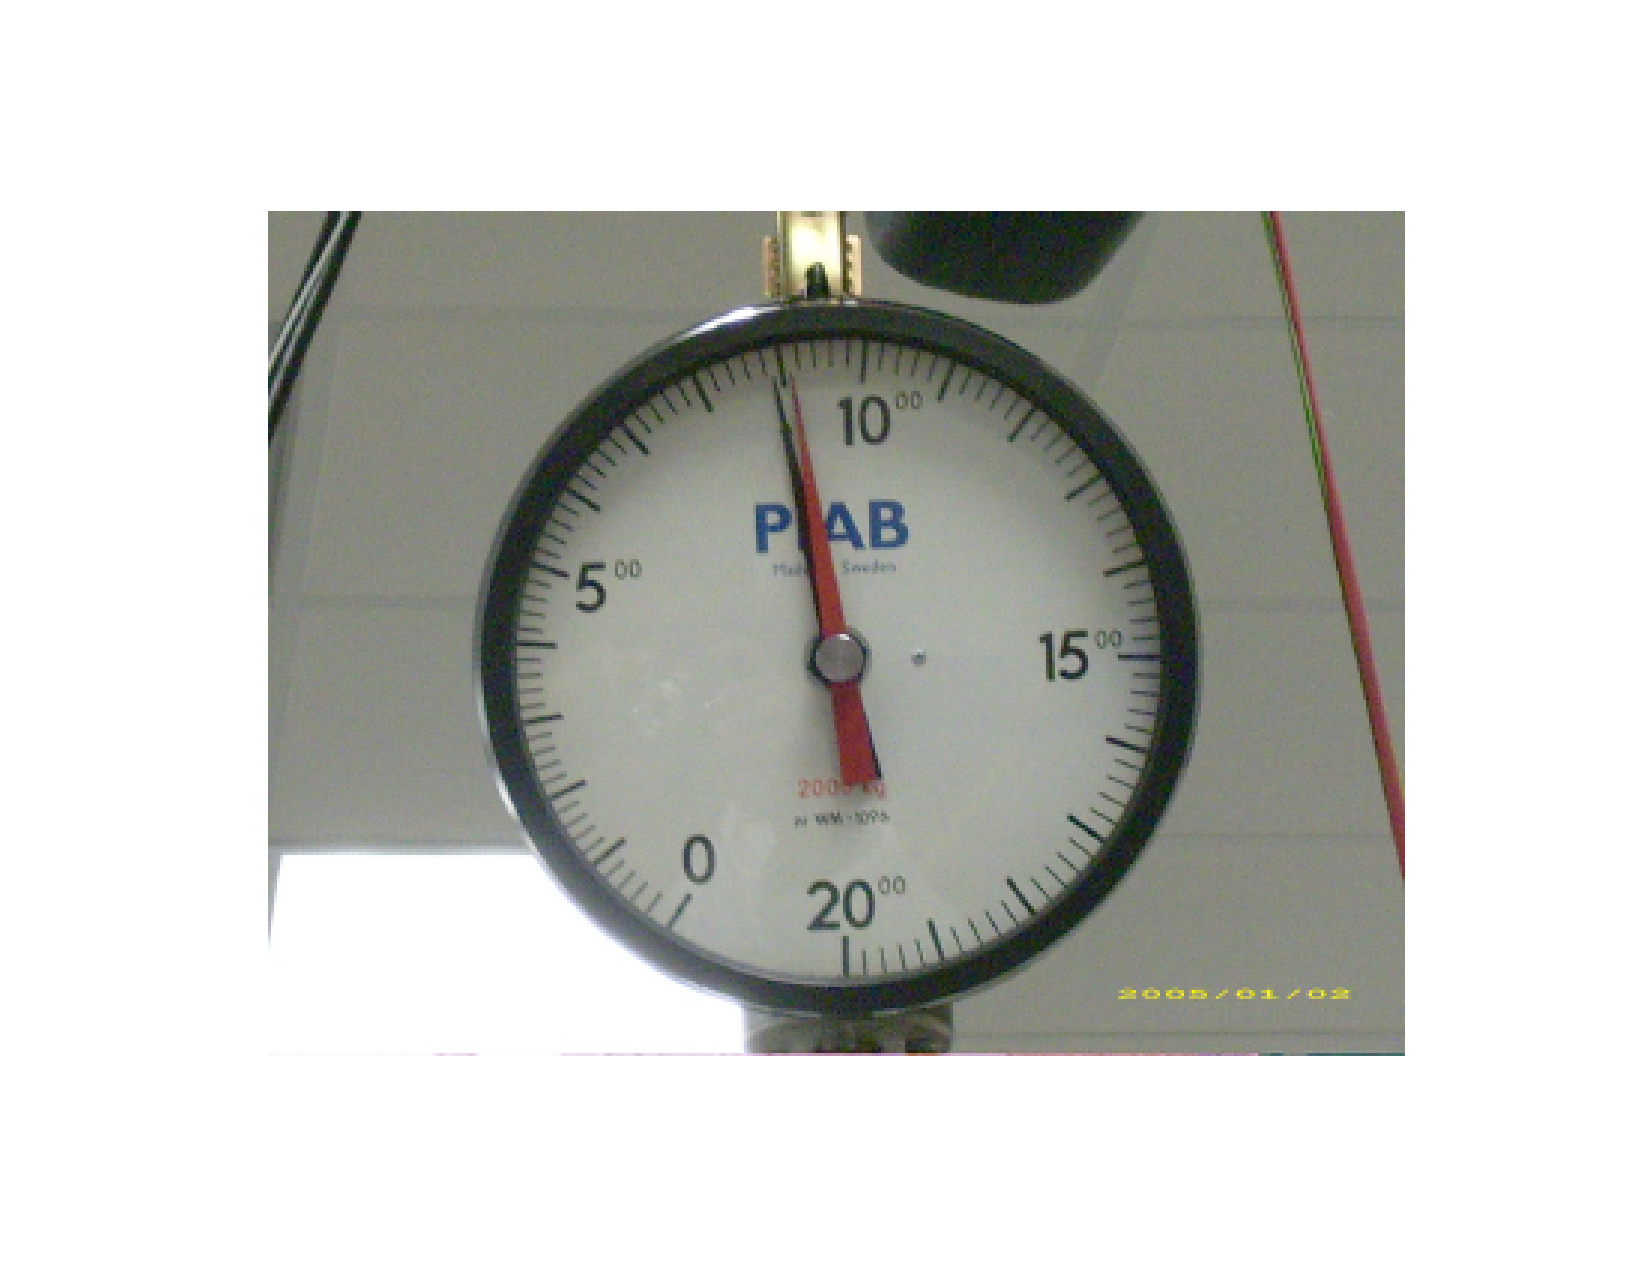
\includegraphics{PIAB.pdf}}        
    \end{tabular}
    \caption{Sketch of the setup used in Torino for the re-calibration
    of the PIAB analog dynamometer (left). Detail of the PIAB display (right.)}
    \label{fig:TOsetup}
  \end{center}
\end{figure}


\begin{figure}[hbtp]
  \begin{center}
  \resizebox{0.7\linewidth}{!}{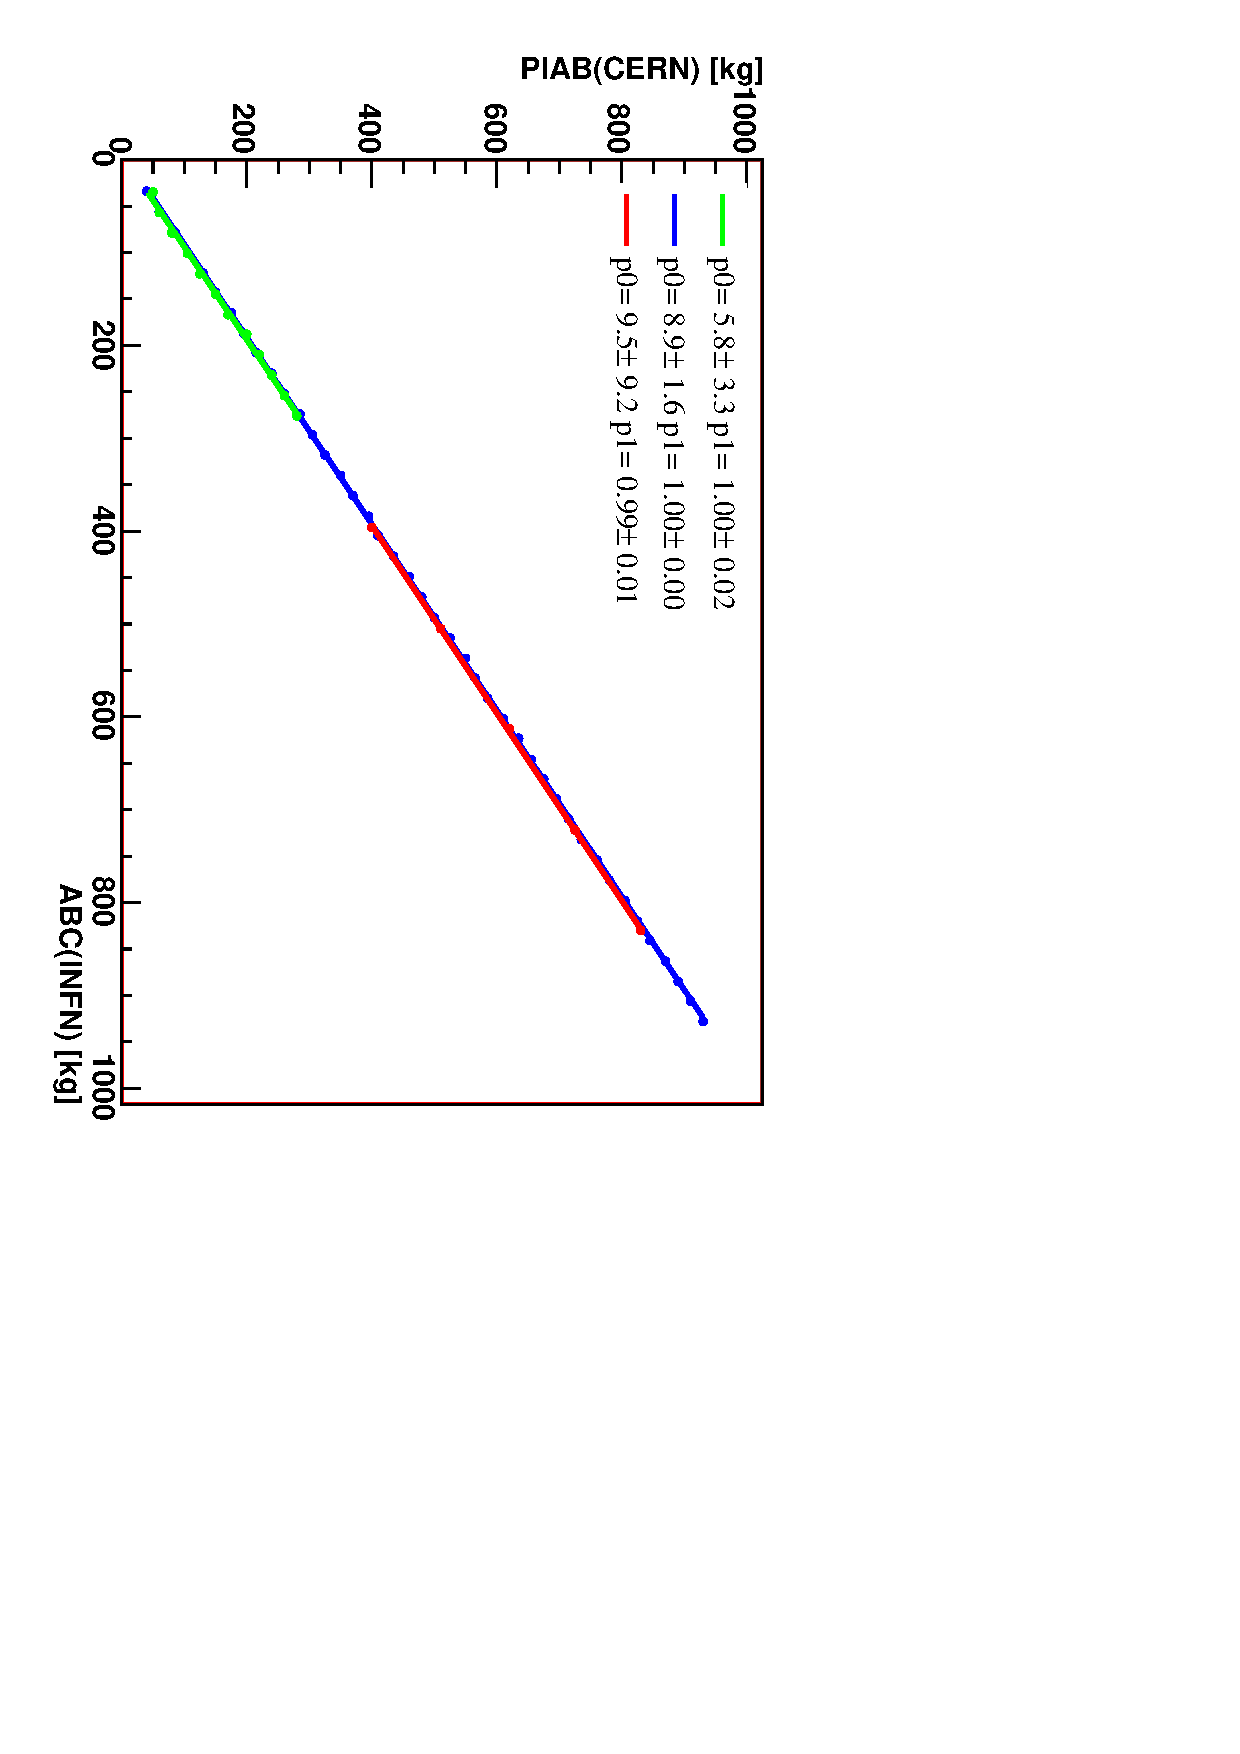
\includegraphics[angle=90]{CalibrazioneFit-CorrTara-Err5kg.pdf}} 
    \caption{Mass of the payload as measured by the PIAB, $m_{\mathrm{PIAB}}$, as a function
    of that measured by the ABC load cell,
    $m_{\mathrm{ABC}}$. A $\pm$5 kg error was assigned to the PIAB
    measurements. Parameters refers to a straight line fit:
    $m_{\mathrm{PIAB}} =p_0 + p_1~\cdot~m_{\mathrm{ABC}}$}
    \label{fig:calib_line}
  \end{center}
\end{figure}


\begin{figure}[hbtp]
  \begin{center}
  \resizebox{0.9\linewidth}{!}{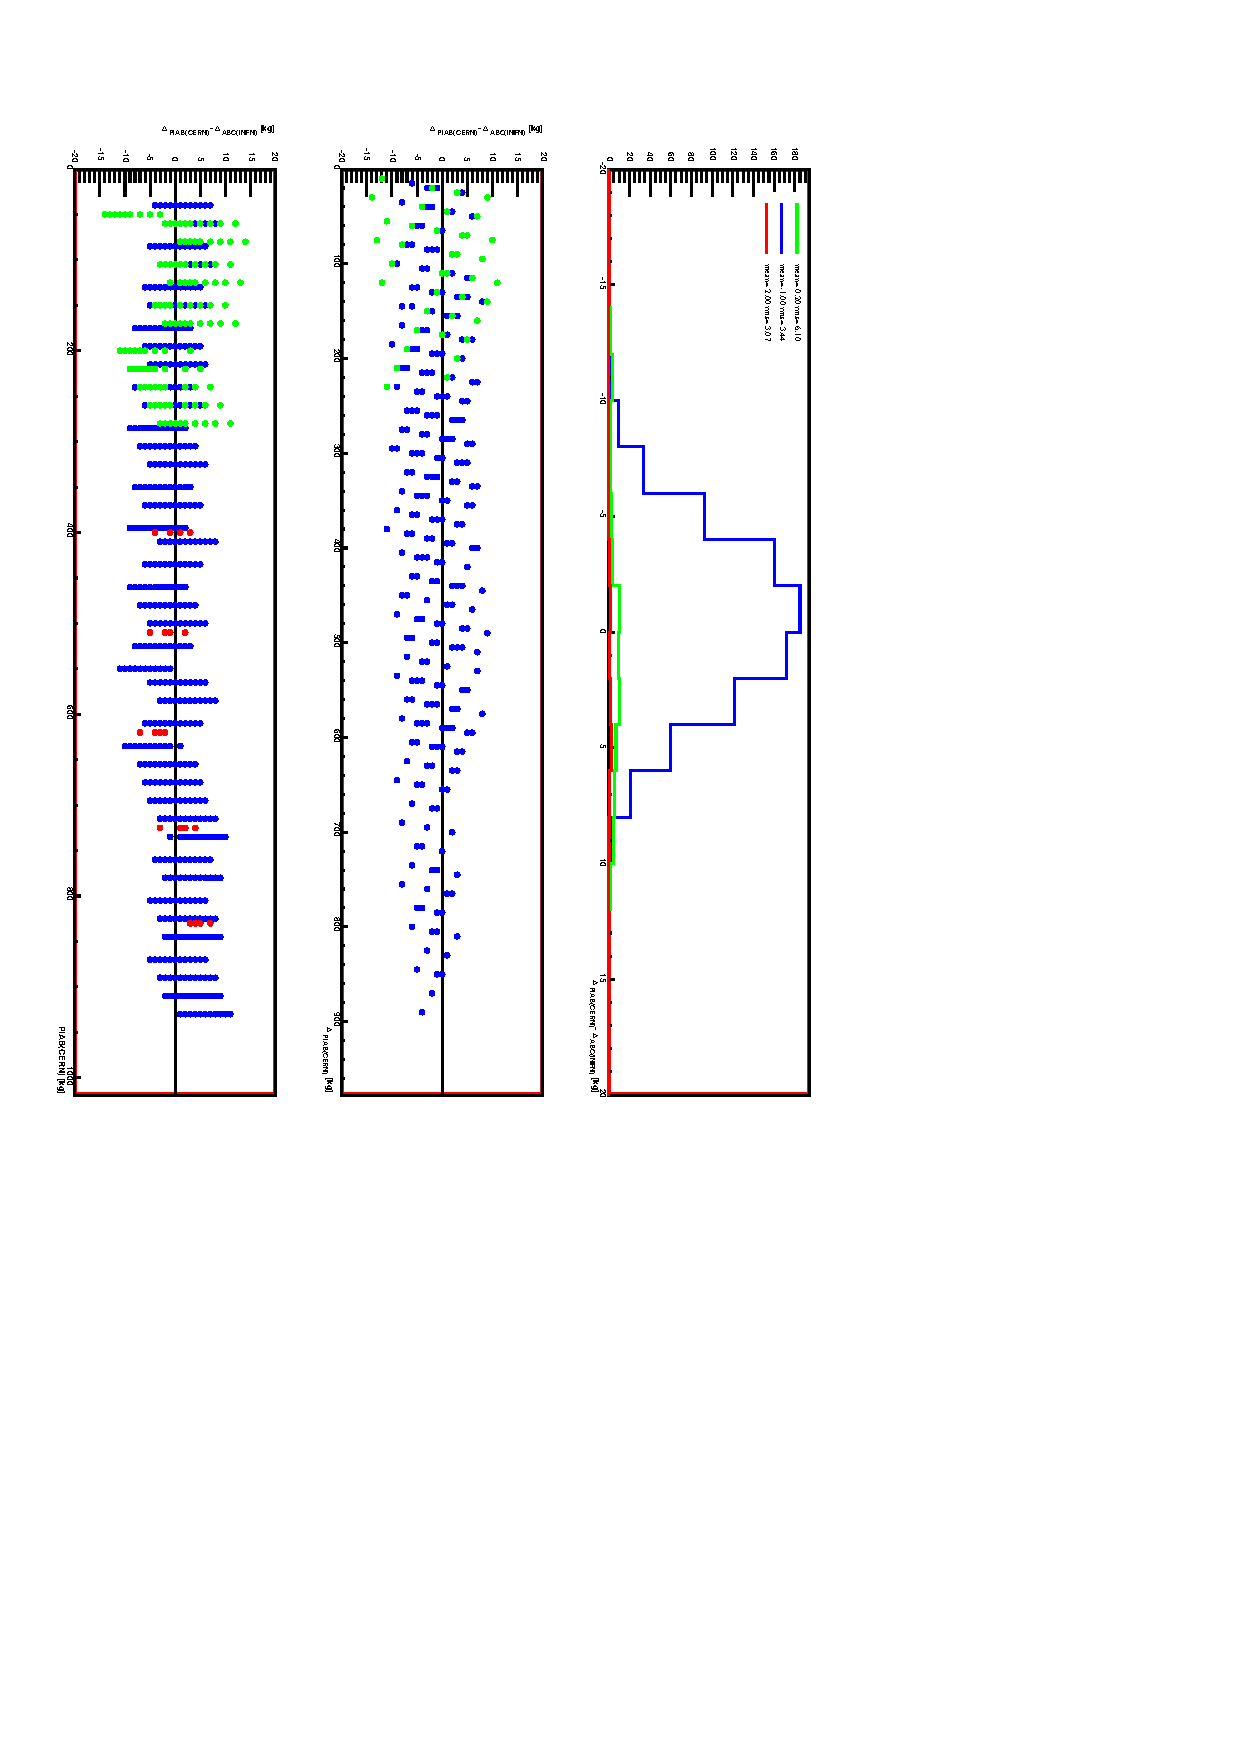
\includegraphics[angle=90]{CalibrazioneDelta-CorrTara-v1.pdf}} 
    \caption{``Double-difference'' distribution
      $\Delta_{\mathrm{PIAB}}-\Delta_{\mathrm{ABC}}$ (top), double
      difference as a function of PIAB ``pseudo-measurements''
      $\Delta_{\mathrm{PIAB}}$ (center)
      and as a function of PIAB measurement (bottom). The entries of the
      last plot are twice those of the first two as the double
      difference value was plot for both the PIAB measurements
      entering in $\Delta_{\mathrm{PIAB}}$.
    }
    \label{fig:calib_delta}
  \end{center}
\end{figure}

\begin{thebibliography}{99}
\bibitem{tdr}
 ``The Tracker Technical Design Report'',             CERN/LHCC 98-6, CMS TDR 5, 15 April 1998;\\
 ``Addendum to the Tracker Technical Design Report'', CERN/LHCC 2000-016, CMS TDR 5 Addendum 1, 21 February 2000.
\bibitem{geant4}
  See {\tt http://geant4.web.cern.ch/geant4}.
\bibitem{ddl}
  See {\tt http://cmsdoc.cern.ch/cms/software/ddd/www}.
\bibitem{rrValid}
  R. Ranieri CMS IN-2007/055, ``The Tracker Geometry Validation Procedure''.
\bibitem{hybrid}
 See {\tt http://www.fynu.ucl.ac.be/he/cms/activities/tracker/FHITfiles/CCTPHybrides.pdf}
\bibitem{piab}
  PIAB Sweden AB, Box 123, 184 22 \AA kersberga, Sweden, 
  {\tt http://www.piab.net}.
\bibitem{abc}
  F.lli AMOS \& C SPA 20093 Cologno Monzese (MI), Italy,
  {\tt http://www.amos.it}.
%  \bibitem {DPG} 
%    E.Migliore and G.Sguazzoni, 
%    {\tt http://indico.cern.ch/conferenceDisplay.py?confId=15247}.
\end{thebibliography}

%%%%%%%%%%%%%%%%%%%%%%%%%%%%%%%%%%%%%%%%%%%%%%%%%%%%
\section{Appendix}
%%%%%%%%%%%%%%%%%%%%%%%%%%%%%%%%%%%%%%%%%%%%%%%%%%%%

\begin{sidewaystable}[p]
  \caption{{\tt TIBModule*} volume list.}
  \label{tab:tib_module}
  \begin{center}
    \begin{tabular}{cccccrr}
         Volume Name                   & Mult. & Solid Name                    & Material Name         & Density [g/cm$^3$]    & Mass [g] & X$_0$ [cm]     \\ 
	 \hline \\
         {\tt TIBModule0BoxFrame}     & 2     & TIBModule0BoxFrame            & Carbon fibre str.     & xxxx          & xxxxxxx   &   \\
	 {\tt TIBModule0*}             &  \multicolumn{4}{r}{\em Total } & {\em  50.6224 g} & \\
	 \hline  \\
         {\tt TIBModule2BoxFrame}     & 2     & TIBModule2BoxFrame            & Carbon fibre str.     & xxxx          & xxxxxxxx  &   \\
	 {\tt TIBModule2*}             &  \multicolumn{4}{r}{\em Total } & {\em  50.6224 g} & \\
	 \hline
    \end{tabular}
  \end{center}
\end{sidewaystable}

\begin{sidewaystable}[p]
  \caption{{\tt TIDModule*} volume list.}
  \label{tab:tid_module}
  \begin{center}
    \begin{tabular}{cccccrr}
         Volume Name                   & Mult. & Solid Name                    & Material Name         & Density [g/cm$^3$]    & Mass [g] & X$_0$ [cm]     \\ 
	 \hline \\
         {\tt TIDModule0RphiKapton}         & 1     & TIDModule0RphiKapton          & T\_TIDModKaptonBox    & 1.25249       & 1.56127   &   \\
         {\tt TIDModule0RphiWafer}          & 1     & TIDModule0RphiWafer           & Silicon               & 2.33          & 0.87528   &   \\
         {\tt TIDModule0RphiActive}         & 1     & TIDModule0RphiActive          & Silicon               & 2.33          & 5.74922   &   \\
         {\tt TIDModule0RphiSideFrame}      & 1     & TIDModule0RphiSideFrame       & Carbon fibre str.     & 1.69          & 5.06954   &   \\
         {\tt TIDModule0StereoSideFrame}    & 1     & TIDModule0StereoSideFrame     & Carbon fibre str.     & 1.69          & 5.06954   &   \\
         {\tt TIDModule0StereoWafer}        & 1     & TIDModule0StereoWafer         & Silicon               & 2.33          & 0.87528   &   \\
         {\tt TIDModule0StereoActive}       & 1     & TIDModule0StereoActive        & Silicon               & 2.33          & 5.74922   &   \\
         {\tt TIDModule0StereoKapton}       & 1     & TIDModule0StereoKapton        & T\_TIDModKaptonBox    & 1.25249       & 1.59622   &   \\ 
         {\tt TIDCoolInsert}                & 4     & TIDCoolInsert                 & TID\_CoolInsert       & 5.46429       & 1.24313   &   \\
         {\tt TIDBottomSpacers}             & 1     & BottomSpacers                 & TID\_Spacer           & 2.9872        & 2.47265   &   \\
         {\tt TIDSideSpacers}               & 2     & SideSpacers                   & TID\_Spacer           & 2.9872        & 0.41671   &   \\
         {\tt TIDModule0RphiPA}             & 1     & TIDModule0RphiPA              & TIBTID\_PA            & 2.74978       & 3.78712   &   \\
         {\tt TIDModule0StereoPA}           & 1     & TIDModule0StereoPA            & TIBTID\_PA            & 2.74978       & 3.66277   &   \\
         {\tt TIDModule0Hybrid}             & 2     & TIDModule0Hybrid              & TIBTID\_Hybrid        & 2.16228       & 2.90542   &   \\
         {\tt TIDModule0BoxFrame}           & 2     & TIDModule0BoxFrame            & Carbon fibre str.     & 1.69          & 1.26877   &   \\
	 {\tt TIDModule0*}             &  \multicolumn{4}{r}{\em Total } & {\em  50.6224 g} & \\
	 \hline  \\
	 {\tt TIDModule1RphiKapton}         & 1     & TIDModule1RphiKapton          & T\_TIDModKaptonBox    & 1.25249       & 1.40514  &  \\
	 {\tt TIDModule1RphiWafer}          & 1     & TIDModule1RphiWafer           & Silicon               & 2.33          & 0.88530  &  \\
	 {\tt TIDModule1RphiActive}         & 1     & TIDModule1RphiActive          & Silicon               & 2.33          & 5.85272  &  \\
	 {\tt TIDModule1RphiSideFrame}      & 1     & TIDModule1RphiSideFrame       & Carbon fibre str.     & 1.69          & 5.17505  &  \\
	 {\tt TIDModule1StereoKapton}       & 1     & TIDModule1StereoKapton        & T\_TIDModKaptonBox    & 1.25249       & 1.44568  &  \\
	 {\tt TIDModule1StereoWafer}        & 1     & TIDModule1StereoWafer         & Silicon               & 2.33          & 0.88530  &  \\
	 {\tt TIDModule1StereoActive}       & 1     & TIDModule1StereoActive        & Silicon               & 2.33          & 5.85272  &  \\
	 {\tt TIDModule1StereoSideFrame}    & 1     & TIDModule1StereoSideFrame     & Carbon fibre str.     & 1.69          & 5.17505  &  \\
	 {\tt TIDCoolInsert}                & 4     & TIDCoolInsert                 & TID\_CoolInsert       & 5.46429       & 1.24313  &  \\
	 {\tt TIDBottomSpacer}              & 1     & BottomSpacers                 & TID\_Spacer           & 2.9872        & 2.47265  &  \\
	 {\tt TIDSideSpacers}               & 2     & SideSpacers                   & TID\_Spacer           & 2.9872        & 0.41671  &  \\
	 {\tt TIDModule1RphiPA}             & 1     & TIDModule1RphiPA              & TIBTID\_PA            & 2.74978       & 4.88096  &  \\
	 {\tt TIDModule1StereoPA}           & 1     & TIDModule1StereoPA            & TIBTID\_PA            & 2.74978       & 4.73305  &  \\
	 {\tt TIDModule1Hybrid}             & 2     & TIDModule1Hybrid              & TIBTID\_Hybrid        & 2.16228       & 2.90542  &  \\
	 {\tt TIDModule1BoxFrame}           & 2     & TIDModule1BoxFrame            & Carbon fibre str.     & 1.69          & 1.26877  &  \\
	 {\tt TIDModule1*}             & \multicolumn{4}{r}{\em Total } & {\em 52.9179 g } & \\
	 \hline	 \\
	 {\tt TIDModule2RphiKapton}     & 1     & TIDModule2RphiKapton          & T\_TIDModKaptonBox    & 1.25249       & 1.36593  &   \\
	 {\tt TIDModule2RphiWafer}      & 1     & TIDModule2RphiWafer           & Silicon               & 2.33          & 0.82666  &   \\
	 {\tt TIDModule2RphiActive}     & 1     & TIDModule2RphiActive          & Silicon               & 2.33          & 5.38995  &   \\
	 {\tt TIDModule2RphiSideFrame}  & 1     & TIDModule2RphiSideFrame       & Carbon fibre str.     & 1.69          & 3.27386  &   \\
	 {\tt TIDCoolInsert}            & 4     & TIDCoolInsert                 & TID\_CoolInsert       & 5.46429       & 1.10160  &   \\
	 {\tt TIDModule2RphiPA}         & 1     & TIDModule2RphiPA              & TIBTID\_PA            & 2.74978       & 1.81506  &   \\
	 {\tt TIDModule2Hybrid}         & 1     & TIDModule2Hybrid              & TIBTID\_Hybrid        & 2.16228       & 2.90542  &   \\
	 {\tt TIDModule2BoxFrame}       & 1     & TIDModule2BoxFrame            & Carbon fibre str.     & 1.69          & 1.64614  &   \\
	 {\tt TIDModule2}          & \multicolumn{4}{r}{\em Total } & {\em 21.6294 g} & \\
	 \hline
    \end{tabular}
  \end{center}
\end{sidewaystable}
%
\pagebreak

\begin{figure}[p]
  \begin{center}
    \resizebox{0.55\linewidth}{!}{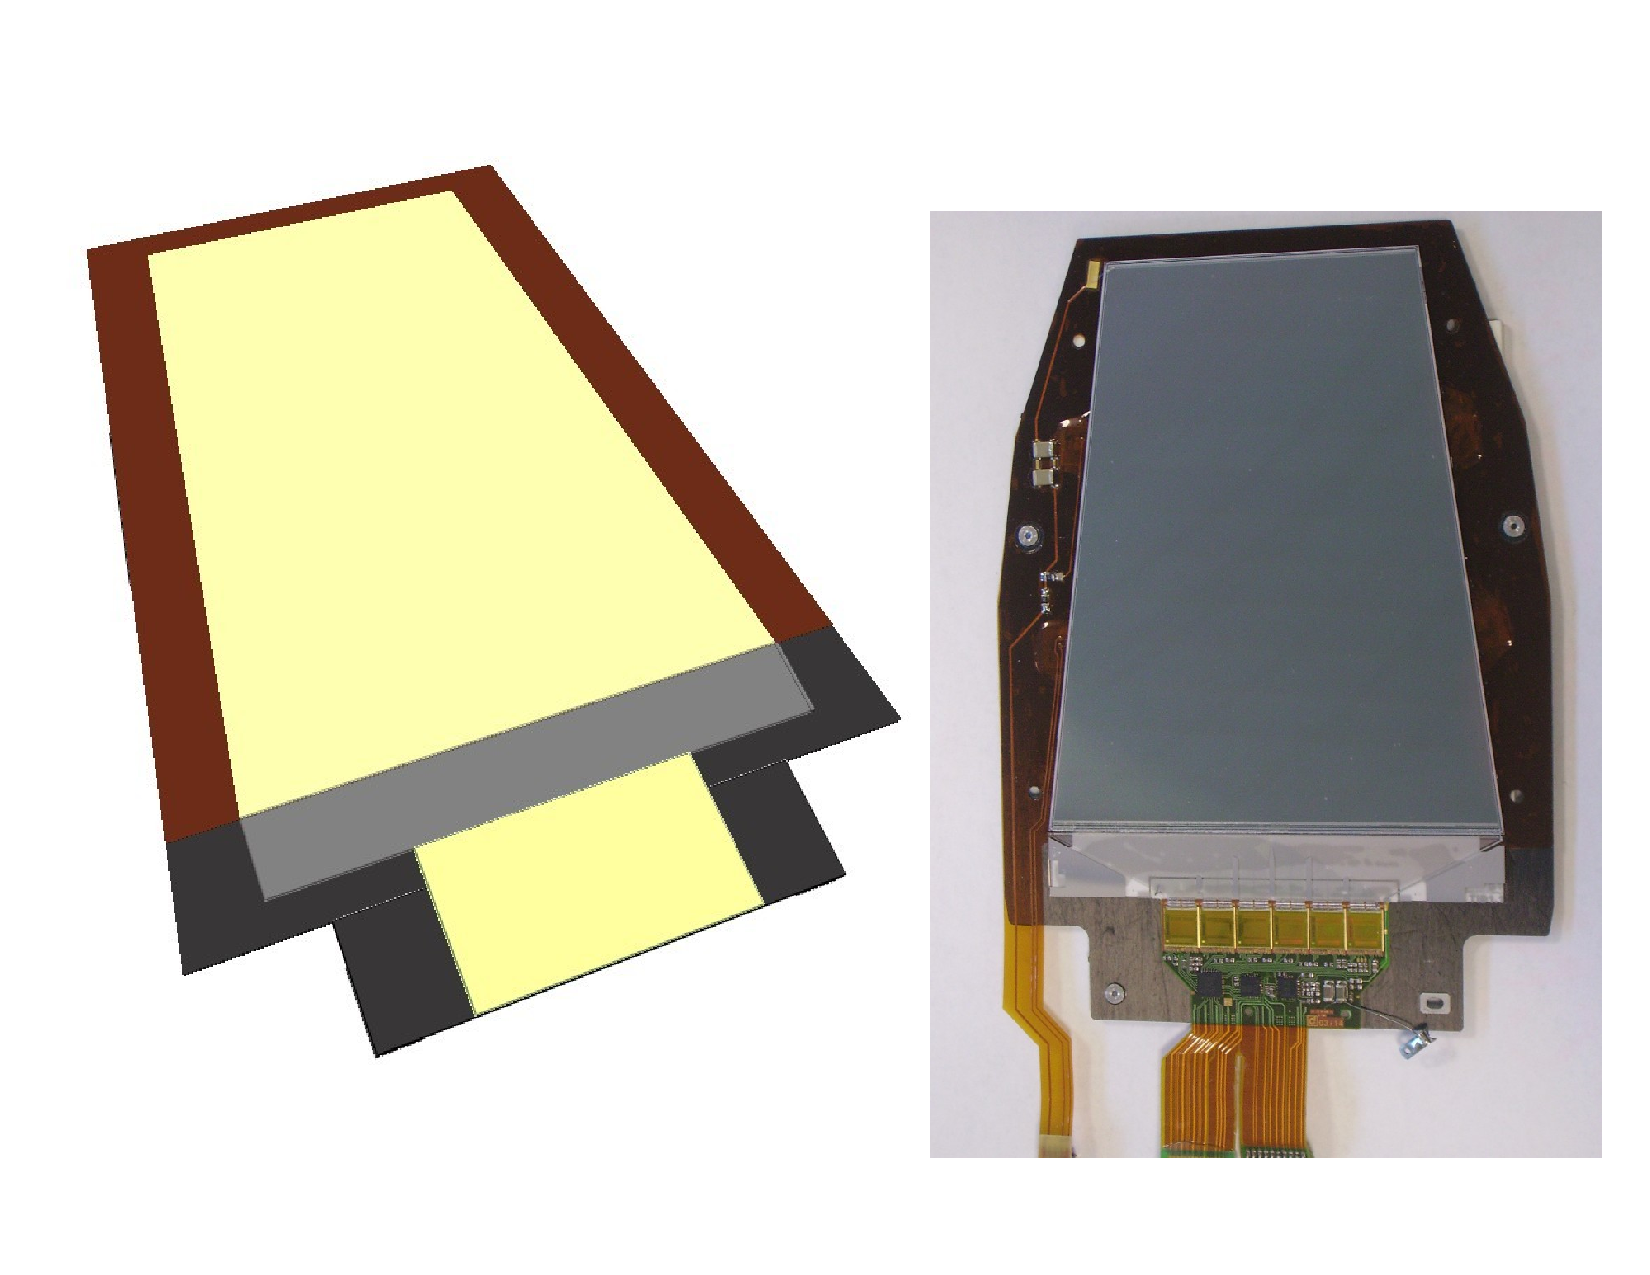
\includegraphics{TIDModule0.pdf}}  \\
    \resizebox{0.55\linewidth}{!}{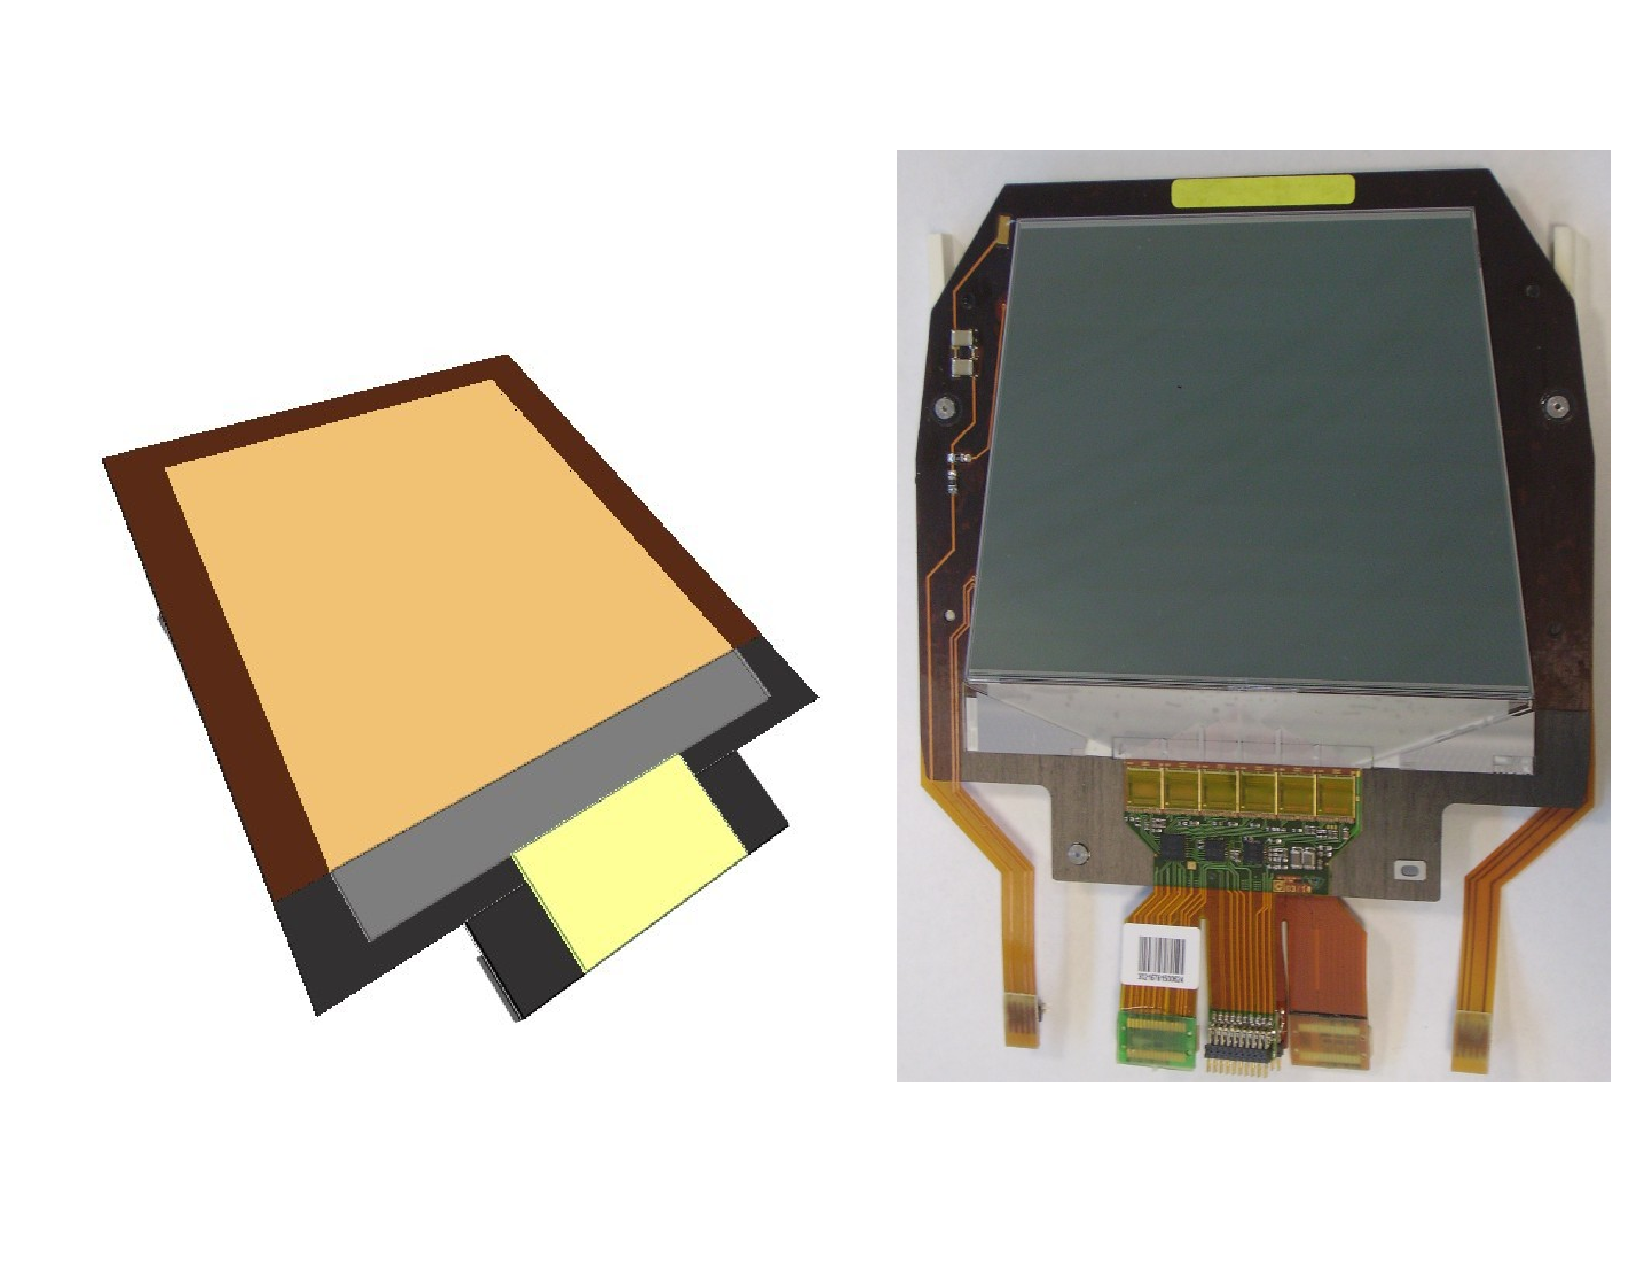
\includegraphics{TIDModule1.pdf}}  \\
    \resizebox{0.55\linewidth}{!}{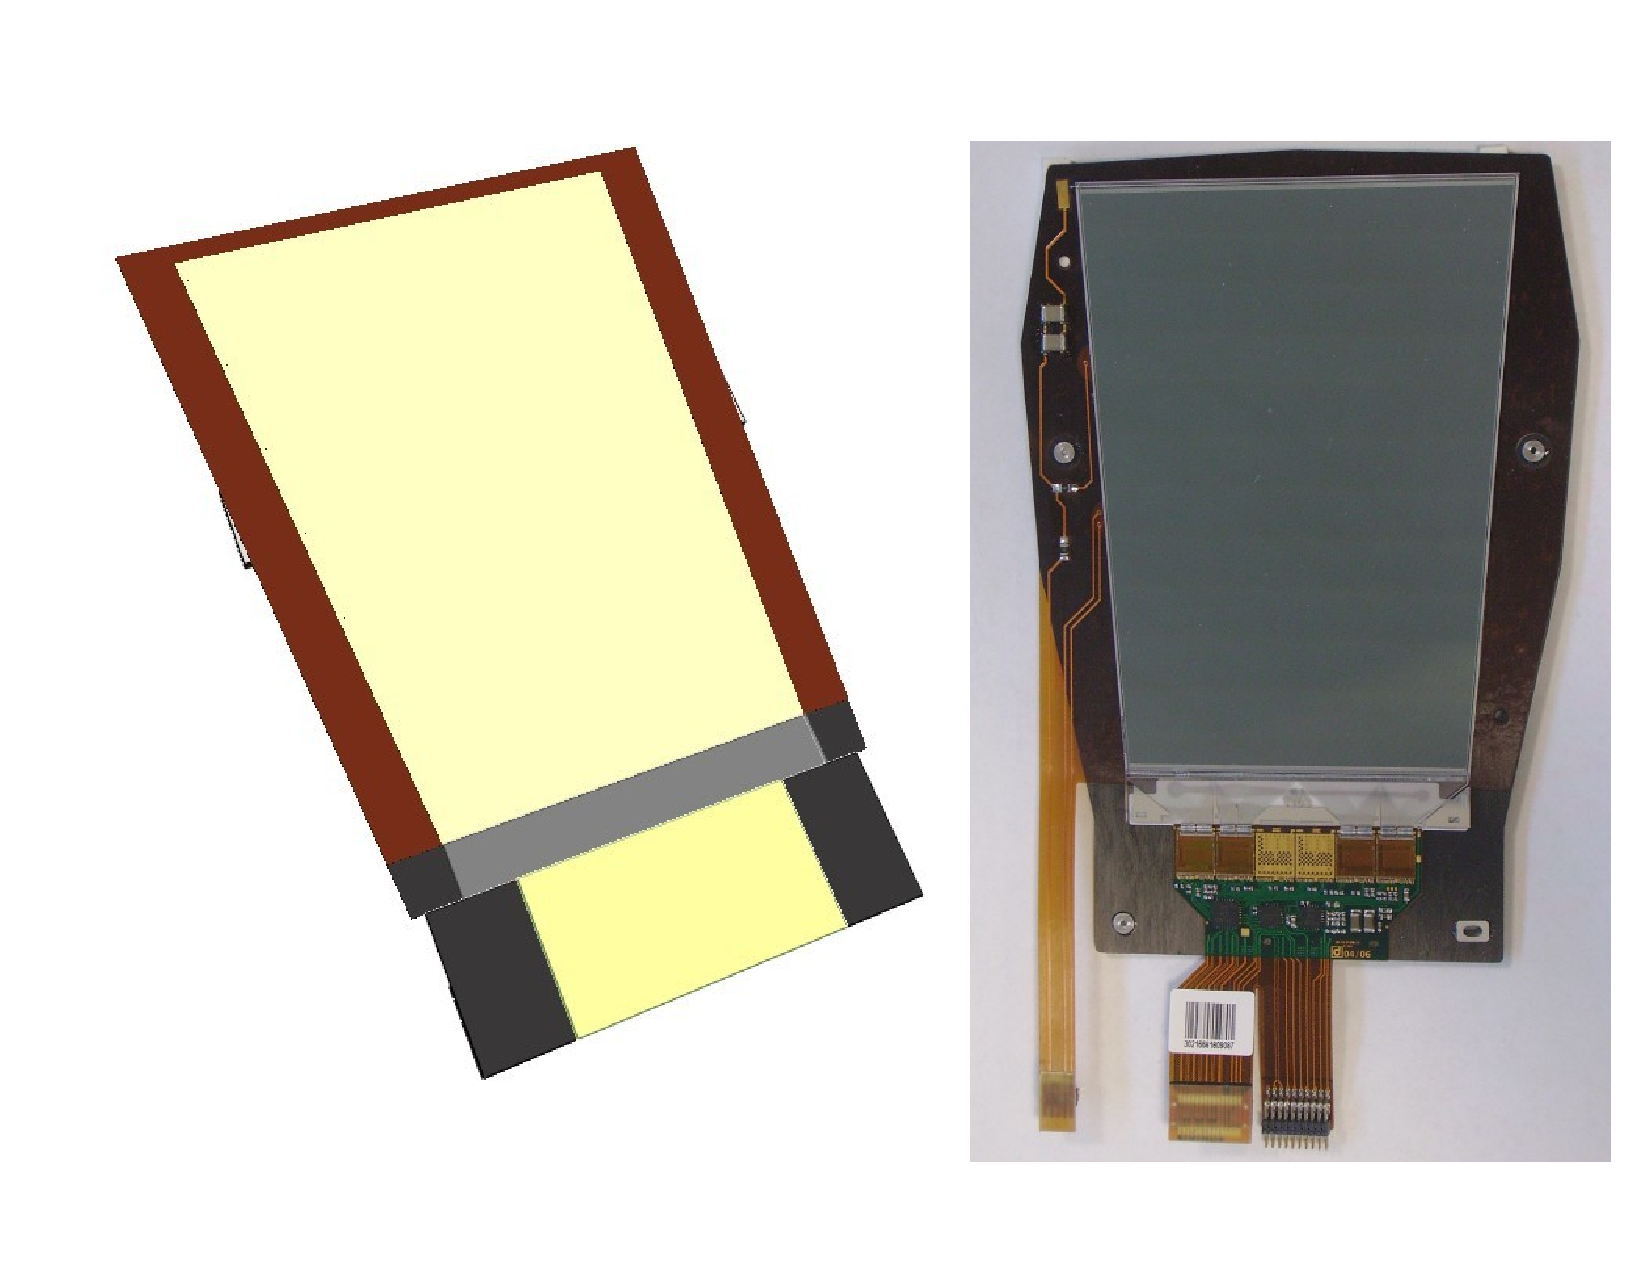
\includegraphics{TIDModule2.pdf}}  \\
    \caption{Modules of the TID}
    \label{fig:TIDModule}
  \end{center}
\end{figure}


 
%------------------------------------------------------------------------------
\pagebreak

\end{document}

% LocalWords:  TODO
